\documentclass{article}

\usepackage{amsmath}
\usepackage{amssymb}
\usepackage{bm}
\usepackage{color}
\usepackage{CJKutf8}
\usepackage{color}
\usepackage{enumitem}
\usepackage{graphicx}
\usepackage{indentfirst}
\usepackage{listings}
\usepackage{mathdots}
\usepackage{tikz}
\usepackage{wasysym}
\usepackage{xcolor}

\setlength{\parindent}{2em}

\usetikzlibrary{shapes,arrows, automata}

\allowdisplaybreaks

\newcommand{\hytt}[1]{\texttt{\hyphenchar\font=\defaulthyphenchar #1}}
\hyphenation{read-Sym-bol re-ad-Space-Tab-New-line str-Tab}

\definecolor{mygreen}{rgb}{0,0.6,0}
\definecolor{mygray}{rgb}{0.5,0.5,0.5}
\definecolor{mymauve}{rgb}{0.58,0,0.82}
%\footnotesize
\lstset{ %
  backgroundcolor=\color{white},   % choose the background color; you must add \usepackage{color} or \usepackage{xcolor}
  basicstyle=\ttfamily,            % the size of the fonts that are used for the code
  breakatwhitespace=false,         % sets if automatic breaks should only happen at whitespace
  breaklines=true,                 % sets automatic line breaking
  captionpos=b,                    % sets the caption-position to bottom
  commentstyle=\ttfamily\color{mygreen},    
                                   % comment style
  deletekeywords={},               % if you want to delete keywords from the given language
  escapeinside={},                 % if you want to add LaTeX within your code
  extendedchars=true,              % lets you use non-ASCII characters; for 8-bits encodings only, does not work with UTF-8
  frame=single,                    % adds a frame around the code
  keepspaces=true,                 % keeps spaces in text, useful for keeping indentation of code (possibly needs columns=flexible)
  keywordstyle=\color{blue},       % keyword style
  language=VHDL,                    % the language of the code
  morekeywords={},                 % if you want to add more keywords to the set
  numbers=left,                    % where to put the line-numbers; possible values are (none, left, right)
  numbersep=5pt,                   % how far the line-numbers are from the code
  numberstyle=\tiny\color{mygray}, % the style that is used for the line-numbers
  rulecolor=\color{black},         % if not set, the frame-color may be changed on line-breaks within not-black text (e.g. comments (green here))
  showspaces=false,                % show spaces everywhere adding particular underscores; it overrides 'showstringspaces'
  showstringspaces=false,          % underline spaces within strings only
  showtabs=false,                  % show tabs within strings adding particular underscores
  stepnumber=1,                    % the step between two line-numbers. If it's 1, each line will be numbered
  stringstyle=\color{mymauve},     % string literal style
  tabsize=2,                       % sets default tabsize to 2 spaces
  title=\lstname                   % show the filename of files included with \lstinputlisting; also try caption instead of title
}

\begin{document}
\begin{CJK*}{UTF8}{gbsn}
\CJKtilde

\title{实验一(2)译码电路设计实验}

\author{计算机1202 张艺瀚\\学号:20123852}
\maketitle

\section{实验目的}
\begin{enumerate}
\item 复习二进制译码器的功能。
\item 学习VHDL语言源程序输入方法。
\item 学习VHDL语言源程序检查和修改。
\item 掌握用VHDL语言设计一个3线-8线译码器的方法。
\item 掌握VHDL语言编辑器的基本操作。
\end{enumerate}

\section{实验原理}
译码为编码的逆过程。它将编码时赋予代码的含义“翻译”过来。实现译码的逻辑电路称为译码器。译码器输出与输入代码有唯一的对应关系。常用的译码器有二进制译码器、二十进制译码器、显示段译码器等等。

3线—8线译码器是二进制译码器的一种。其输人为一组三位二进制代码,而输出则对应—路高、低电平信号。图~\ref{fig: afig} 示出了3线—8线译码器74138的逻辑图。

其中A,B,C为三位二进制代码输人端。Y0-Y7是八个输出端,G1, G2A, G2B 为三个输入控制端。只有当G1=1,G2A=0,G2B=0时,译译码器才处于工作状态。否则,译码器将处在禁止状态,所有输出端全为高电平。其对应的真值表如图~\ref{fig: bfig} 所示。

\begin{center}
\begin{figure}[h!]
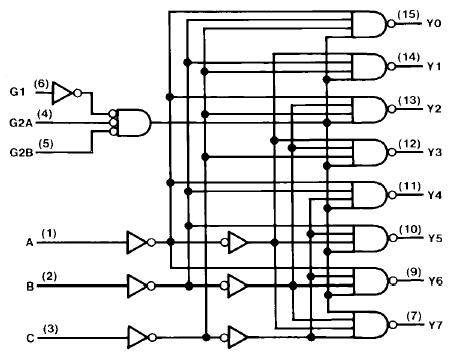
\includegraphics[width=\textwidth]{1.jpg}
\caption{74138译码器的逻辑图}
\label{fig: afig}
\end{figure}
\end{center}

\begin{center}
\begin{figure}[h!]
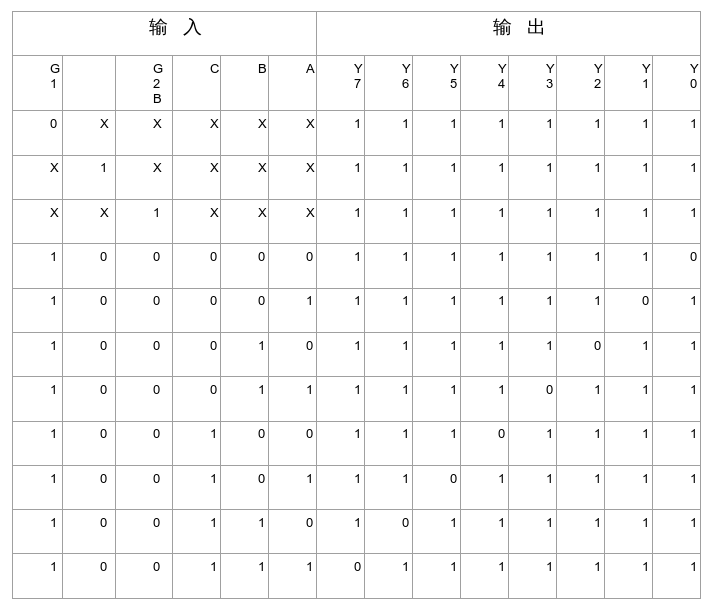
\includegraphics[width=\textwidth]{2.jpg}
\caption{74138译码器的真值表}
\label{fig: bfig}
\end{figure}
\end{center}

\section{实验内容}
\begin{enumerate}
\item 本实验给出了有错误的3线—8线译码器的VHDL程序,请采用VHDL编辑器,修改调试程序。
\item 仿真3线—8线译码器的设计。
\end{enumerate}

\section{实验设备}
\begin{enumerate}
\item 清华同方PⅣ 2.4G/256M60G
\item ISE 6.2i—Windows软件系统
\end{enumerate}

%\section{实验步骤}

\section{实验程序}
\begin{center}
\begin{lstlisting}[caption = {74138译码器的代码清单}, label = {lst: aonelst}]
library IEEE;
use IEEE.STD_LOGIC_1164.ALL;
use IEEE.STD_LOGIC_ARITH.ALL;
use IEEE.STD_LOGIC_UNSIGNED.ALL;

--  Uncomment the following lines to use the declarations that are
--  provided for instantiating Xilinx primitive components.
--library UNISIM;
--use UNISIM.VComponents.all;

entity program is
port(a: in std_logic;
	b: in std_logic;
	c: in std_logic;
	g1: in std_logic;
	g2a: in std_logic;
	g2b: in std_logic;
	y: out std_logic_vector(7 downto 0));
end program;

architecture Behavioral of program is
signal d_in: std_logic_vector(2 downto 0);
begin
d_in<=c&b&a;
process(d_in)
begin
if(g1='1' and g2a='0' and g2b='0')then
	case d_in is
	when "000"=>y<="00000001";
	when "001"=>y<="00000010";
	when "010"=>y<="00000100";
	when "011"=>y<="00001000";
	when "100"=>y<="00010000";
	when "101"=>y<="00100000";
	when "110"=>y<="01000000";
	when "111"=>y<="10000000";
	when others=>NULL;
	end case;
else
	y<="11111111";
end if;
end process;
end Behavioral;
\end{lstlisting}
\end{center}

\section{仿真结果}
\begin{center}
\begin{figure}[h!]
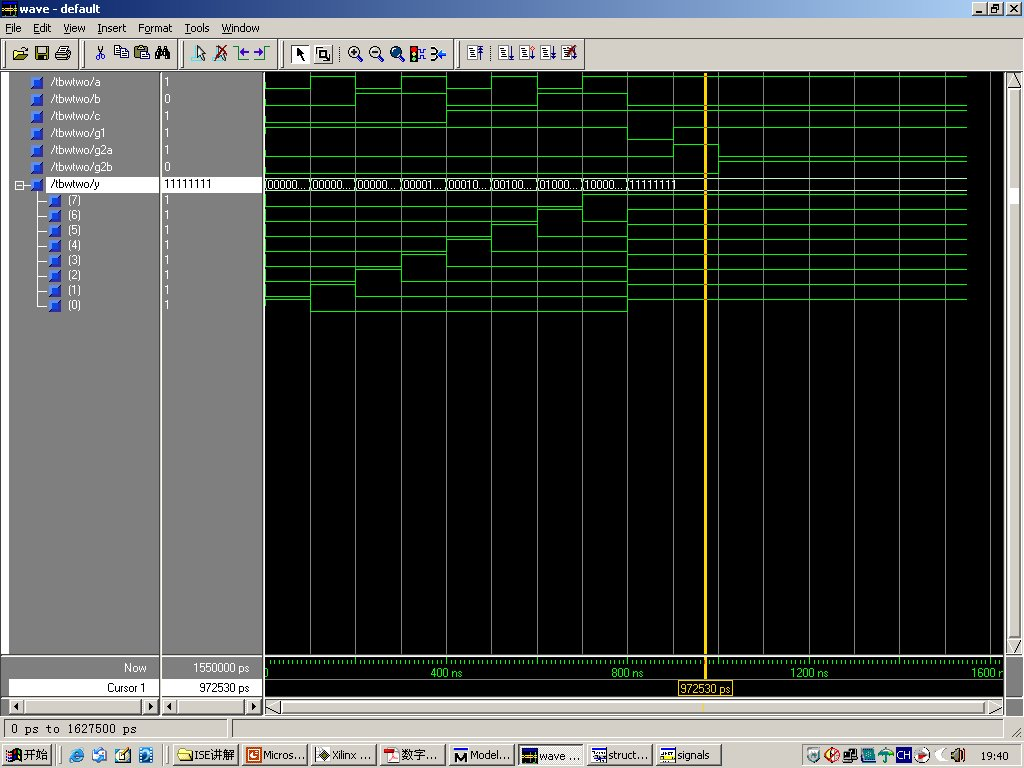
\includegraphics[width=\textwidth]{3.jpg}
\caption{74138译码器的仿真波形图}
\label{fig: cfig}
\end{figure}
\end{center}

\end{CJK*}
\end{document}
